\section{Qt}
%short introduction to the chapter
Qt, pronounced "cute", is an open source cross-platform framework, mostly used for GUI(graphical user interface) programming. Qt has an easy to (re)use API(application programming interface), which in return gives high developer productivity. QT is C++ class library, hence new developers using Qt should have some understanding of C++.
This chapter introduces terminologies used in Qt, and tries to give some general insight to how Qt operates and works regarding GUI development. For more information please refer to \cite{QtDocumentation}.

%Maybe something about licencing and version used.


%somewhere here should the "simple" inheritance diagram be.

\subsection{Qt Class Hierarchy and Object Model}
\label{sec:QtClassHierarchyAndObjectModel}
Qt broadly uses inheritance to create subclasses of instances in a natural way. QObject is the most basic class in Qt, see figure~\ref{fig:QtHeirachy}. A lot of classes inherit from QObject, like QWidget, which is the base of all user interface objects. 

\begin{figure}[h]
	\centering
	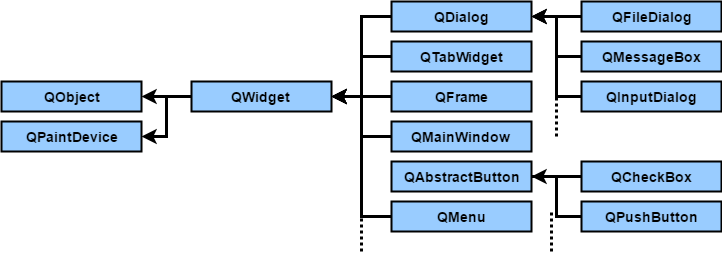
\includegraphics[scale=0.55]{Figures/QtHierachy.png}
	\caption{Illustration of some of the hierarchy that Qt is structured as. A complete illustration would be massive an span hundreds of classes.}
	\label{fig:QtHeirachy}
\end{figure}

C++ offers efficient runtime for a object oriented scheme, but lacks in regard to flexibility due to the static nature of the C++ Object Model. Qt has implemented the QObject as the hearth of the Qt Object Model, which preserve the efficient runtime while also offering more flexibility for the GUI domain. The Qt Object Model is implemented with standard C++ techniques. Some of the features that the Qt Object Model adds are e.g.

\begin{itemize}
\item Inter-Object Communication called Signal and Slots in the Qt Object Model. This topic is expanded upon in section~\ref{sec:signalandslots}.
\item Object Trees which structures ownership of objects in a natural fashion. This topic is expanded upon in section~\ref{sec:qwidgets}.
\end{itemize}

\subsubsection{The Meta-Object System}
\label{sec:TheMetaObjectSystem}
Due to the Qt Object Model the Meta-Object System was in turn created, which on the bottom line provides the Signal and Slots for inter-object communication and other features from the the QT Object Model. The Meta-Object System is based on three things:
\begin{enumerate*}[label={\alph*)},font={\color{red!50!black}\bfseries}]
\item the QObject class
\item the Q\_OBJECT macro and
\item the Meta-Object compiler(moc).
\end{enumerate*}
Each QObject or subclass of QObject has an instance of QMetaObject created to hold the meta-data information, e.g. the name of the class or the class's meta-methods(signal, slots and other member functions). The Q\_OBJECT macro helps and defines the meta data for the moc at compile time. Please refer to figure~\ref{fig:QtC++BuildProcess} to see influence of the Meta-Object System in compile time.

\begin{figure}[h]
	\centering
	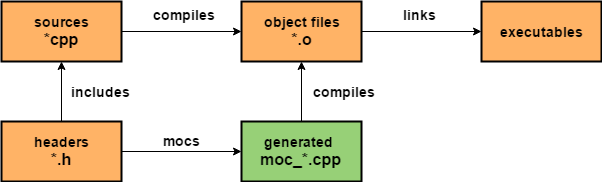
\includegraphics[scale=0.55]{Figures/QtC++BuildProcess.png}
	\caption{This figure shows how the the Meta-Object System is integrated at compile time. The yellow boxes indicate the normal C++ compiling procedure, whereas the green box is the added moc, which is compiled into the object files}
	\label{fig:QtC++BuildProcess}
\end{figure}

\subsection{QWidgets}
\label{sec:qwidgets}
QWidget is the base of all user interface objects(buttons, menus etc.). QWidget handles all events from the system the application is running on. In Qt, events are QEvent objects which is created upon outside activity (like a click on a mouse). Subclasses of QEvent involve more parameters to characterize a certain event, e.g. mousePressEvent(QMouseEvent* event). The event object is then sent to a specific QWidget object (maybe a button) and the QWidget handles the event with the according event handler.\\

As mentioned in~\ref{sec:QtClassHierarchyAndObjectModel} ownership of objects is structured in a tree, this means that a QWidget can have QWidget's within it self, see figure~\ref{fig:QWidgetExample}. It is the parent's responsibility to delete all it's children, if the parent instance is deleted. A QWidget with no parent is called a top-level widget, which means the QWidget is an independent window. An instance like QWidget subclass QDialog(a pop up dialog window) is a top-level widget. QDialog can be instantiated with a parent, but the QDialog is still a top-level widget in this case, though the position of the dialog window is now centred relative to the parent.

\begin{figure}[h]
	\centering
	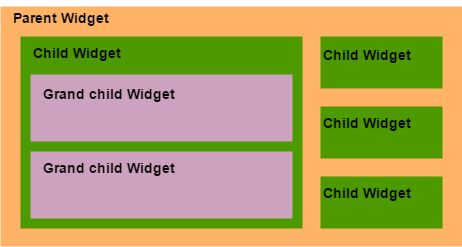
\includegraphics[scale=0.55]{Figures/QWidgetExample.png}
	\caption{Qt structures ownership of objects in a parent child relationship. The diagram shows a parent widget with various child widgets in a layout, more on layouts in section~\ref{sec:QLayout}.}
	\label{fig:QWidgetExample}
\end{figure}

When a QWidget is used as a container to hold and group children, the QWidget is called a composite widget. A parent widget is clipped to the size that it children requires, though this can be changed in the widget's size policy. 

\subsubsection{QMainWindow}
QMainWindow is a subclass of QWidget, and is very essential to a Qt GUI application, since the QMainWindow is a framework for the application user interface. As seen on figure~\ref{fig:QMainWindowExample} a QMainWindow can have a menu bar widget, toolbar bar widgets, docked widgets and a status bar widget, though a QMainWindow must have a central widget, even if that widget is only a empty placeholder. 

\begin{figure}[h]
	\centering
	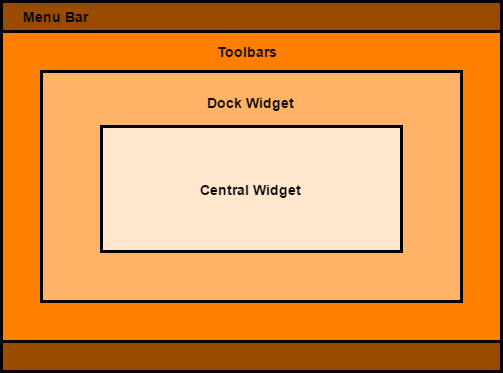
\includegraphics[scale=0.55]{Figures/QMainWindowExample.png}
	\caption{This figure shows how a QMainWindow object looks like. RWS uses QMainWindow as the main application widget.}
	\label{fig:QMainWindowExample}
\end{figure}

QMainWindow is usually a good class to use as the framework for an GUI application, though it is optional whether to use it or not. In the case of RWS, QMainWindow is used, and figure~\ref{fig:QMainWindowExample} nicely reflect the structure of RWS' GUI, where the central widget is a custom subclassed QWidget using Qt GUI modules providing classes for OpenGL integration for graphic rendering. The central widget of RWS will also be referred to as the 3D View. Various plug-ins to RWS are available to be docked in the docking area, or to be top-level windows (more on plug-ins in section~\ref{sec:plugin}) and tool bars and a menu bar are present as well for use.

\subsubsection{QLayout}
\label{sec:QLayout}
QLayout is a subclass of QObject and QLayoutItem and is the base class of geometry managers. QLaoyt and it's subclasses are managers for the layout of a group of widget laid out in an application. All QWidget subclasses can use layouts to manage it's children e.g. figure~\ref{fig:QWidgetExample} uses the parent widget as composite widget with two composite children. The parent on figure~\ref{fig:QWidgetExample} use a QHBoxLayout, which lines the child widgets horizontally and makes each child fill one box. The children then has their own QVBoxLayout, which lines their children (grand children) vertically and assign each of those their own box as well. Figure~\ref{fig:QLayoutCode} shows how an implementation of five arbitrary widgets laid in the layout as in figure~\ref{fig:QWidgetExample}.

\begin{figure}[h]
\centering
\lstset{language=C++} 
\begin{lstlisting}[frame=single]  
QWidget* parent = new QWidget();  			//Parent widget
QHBoxLayout* pL = new QHBoxLayout();		//Layout of the parent widget
QWidget* cL = new QWidget(parent); 			//Left child widget
QVBoxLayout* cLL = new QHBoxLayout();		//Layout of left child widget
QWidget* cR = new QWidget(parent); 			//Right child widget
QVBoxLayout* cRL = new QHBoxLayout();		//Layout of right child widget
pL->addWidget(cR); pL->addWidget(cR);		//add children to layout
parent->setLayout(pL);						//set layout
QWidget* b1 = new QWidget(cL), b2 = new QWidget(cL), b3 = new QWidget(cR),
		 b4 = new QWidget(cR), b5 = new QWidget(cR); //create grandchildren
cLL->addWidget(b1), cLL->addWidget(b2);	//grand children added to layout
cL->setLayout(cLL);					//set layout
cRL->addWidget(b3), cRL->addWidget(b3), cRL->addWidget(b5);				 
cR->setLayout(cRL);			 
\end{lstlisting}
\caption{This code shows how to make a composite widget with a layout like figure~\ref{fig:QWidgetExample}.}
\label{fig:QLayoutCode} 	
\end{figure}


\subsection{Signal and Slots}
\label{sec:signalandslots}
Signals and slots are one of the more unique features provided by Qt, compared to other GUI frameworks. Signals and slots are used for inter-object communication, and it is made possible by the meta-object system (see section~\ref{sec:TheMetaObjectSystem}).The Signal and Slot mechanism is similar to callbacks, which basically are function pointers passed as arguments to other code, that is expected to call back the argument at some time. Qt made signals and slots instead of using callbacks to provide simplicity and ensure type-correctness of callback arguments.

The Signal and Slot mechanism, see figure~\ref{fig:SignalAndSlots}, can be thought of as an implementation of the Observer Pattern PUT SOME REFERNCE HERE. A widget or object (the subject) can emit signals when particular events occurs, these signals can then be connected to slots of other objects (the observers). This means, when an object emits a signal, the connected object(s) slot will be called and executed. A signal can be connected to as many slots is needed, and slot vice versa. A slot does not know if it has a signal connected to it, and an object does not know if anything receives its signals.   

\begin{figure}[h]
	\centering
	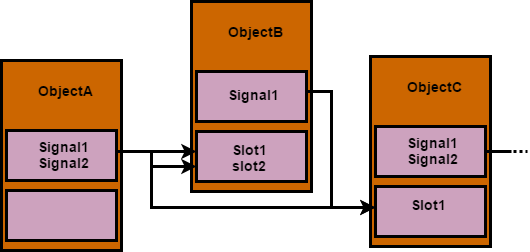
\includegraphics[scale=0.55]{Figures/SignalsAndSlots.png}
	\caption{This figure shows how three objects can signal events to a specific slot of another object.}
	\label{fig:SignalAndSlots}
\end{figure}

Qt widgets comes with many signals and slots for easy use, but these widgets can of course be subclassed to add our own signals and slots. Signals are public access functions and can be emitted from anywhere. Slots are normal member functions, though the they have to be defined in the .h file as seen on figure~\ref{fig:subClassQWidget}, so the moc can find them. Likewise signals are defined in the .h file.

\begin{figure}[h]
\centering
\lstset{language=C++} 
\begin{lstlisting}[frame=single] 
class object : public QWidget
{
	Q_OBJECT
public:
	object(QWidget *parent = 0);
	~object();
private slots:
	void slot1();
signals:
	void signal1();
}
\end{lstlisting}
\caption{This is the .h file for an arbitrary object subclass of QWidget. It shows how the object can be constructed with a parent. The object also has the macro Q\_OBJECT the moc to define the slot and signal.}
\label{fig:subClassQWidget} 	
\end{figure}

The Signal and Slot mechanism is independent of any GUI event loop. That means that any QThread, inherited by QObject, runs its own event loop and  has no influence on the signal/slot mechanism, though it should be noted that using direct connections, where sender and receiver live in different threads, can be unsafe.

\begin{figure}[h]
\centering
\lstset{language=C++} 
\begin{lstlisting}[frame=single]  
connect(ObjectA, SIGNAL(Signal1()), ObjectB, SLOT(Slot1()));
connect(ObjectA, SIGNAL(Signal2()), ObjectB, SLOT(Slot2()));
connect(ObjectA, SIGNAL(Signal1()), ObjectC, SLOT(Slot1()));
\end{lstlisting}
\caption{An example of how to connect ObjectA to Slot1 and Slot2 of ObjectB and Slot1 of ObjectC from figure~\ref{fig:SignalAndSlots}.}
\label{fig:connect} 	
\end{figure}


\subsection{Plug-in}
\label{sec:plugin}
Qt has a low-level API for extending Qt applications. This means that it is possible to make a custom widget(plug-in), which can dynamically be loaded in and out of the application. E.g. if the application lacks a user functionality, then it can be written without changing the main application. This is nice, because then third-party developers can easily extend the application while keeping it separate from the source code of the application.\\

Qt plug-ins are stored as shared libraries (.so for linux), and are loaded on runtime with QPluginLoader. Though to extend a application with plug-ins, the application need to define a set of interfaces (these need to pure virtual functions), so that the plug-ins can communicate with the application. Further more, the moc should be made aware of the interface with Q\_DECLARE\_INTERFACE() in the header file of the defined set of interfaces. Lastly qobject\_cast() should be used to test whether a plug-in interfaces correctly to the application. See figure~\ref{fig:plugin} for an illustration of how RWS uses plug-ins.\\


\begin{figure}[h]
	\centering
	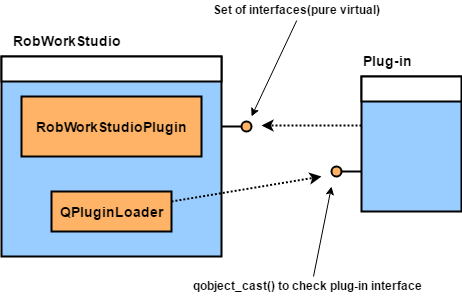
\includegraphics[scale=0.55]{Figures/pluginRWS.png}
	\caption{RWS has a class RobWorkStudioPlugin to define the interfaces for plug-ins to RWS. The plug-in is then loaded into RWS, with the QPluginLoader class, and tested for interface compatibility with qobject\_cast().}
	\label{fig:plugin}
\end{figure}

Creating a plug-in involves declaring the plug-in class inherited by QObject and the interfaces the plug-in wants to provide. The plug-in then need to use the Q\_INTERFACES() macro to tell the moc about the interfaces. With the Q\_PLUGING\_METADATA() macro the plug-in is exported, the macro instantiates the meta-data. The build process of the plug-in should then be appropriate using any preferred method. (E.g. CMake.)







